\documentclass[11pt, a4paper,twocolumn]{jarticle}
\usepackage[dvipdfmx]{graphicx}
\begin{document}
%=============================================================
\section{Digital circuit ($6^{th} day$)}
\subsubsection{Purpose}
Flip-flop(FF)回路は回路状態を記憶でき,電気回路の前の入出力状態に反応する複雑な機能を実現できるため,デジタル回路において重要な要素である.
FFの基礎的な動作を理解するためにreset-set FFを作り,FFの応用としてのデジタルカウンターの動作を調べる.
\subsection{Equipment}
\begin{itemize}
    \item 前回の実験と同様のもの
    \item CMOS NAND IC 74HC00
    \item CMOS counter IC 74HC4040
    \item printed circuit boads
    \item push switchs
\end{itemize}
\subsubsection{Procedure}
図\ref{fig:15}に示すようにリセット・セットFF回路を制作し入力
$\overline{S},\overline{R}$の値ををそれそれ変えながら出力電圧の値を計測する.
その計測結果を表にまとめる.

次に図\ref{fig:16}に示すようにデジタルカウンター回路を作り入力電圧をファンクションジェネレーターを用いて矩形波とし,その動作を確認する.
入出力電圧をオシロスコープで測定したのち,そのグラフを作りデジタルカウンターの動作について考える.

\begin{figure}[htbp]
 \begin{center}
  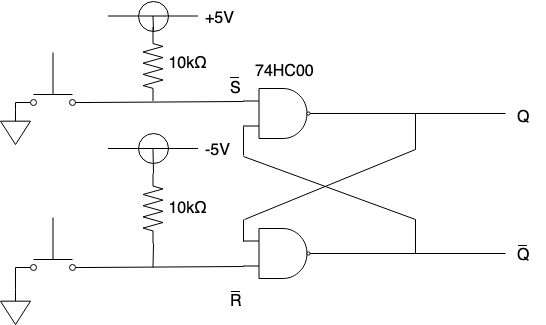
\includegraphics[width=0.8\linewidth]{fig15.png}
 \end{center}
 \caption{reset-set FF回路}
 \label{fig:15}
\end{figure}

\begin{figure}[htbp]
 \begin{center}
  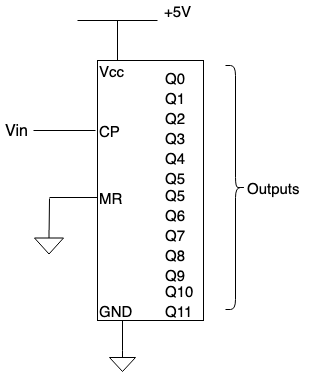
\includegraphics[width=0.8\linewidth]{fig16.png}
 \end{center}
 \caption{Diagram of digital counter}
 \label{fig:16}
\end{figure}
\newpage

\subsubsection{Result}
まずリセットセットFF回路の実験における真理表を表\ref{tab:2}に示す.

\begin{table}[htb]
  \begin{center}
    \caption{reset-set FF回路の真理表}
    \begin{tabular}{c c c c} \hline
         $\overline{S}$ & $\overline{R}$ & $Q_{n+1}$ & $\overline{Q}_{n+1}$ \\ \hline \hline
         1 & 1 & 1 & 1 \\ \hline
         0 & 1 & 0 & 1 \\ \hline
         1 & 0 & 1 & 0 \\ \hline
         0 & 0 & $Q_{n}$ & $\overline{Q}_{n}$ \\ \hline
    \end{tabular}
    \label{tab:2}
  \end{center}
\end{table}

次にデジタルカウンター回路のQ1からQ5まで測定した結果を以下に示す.

\begin{figure}[htbp]
 \begin{center}
  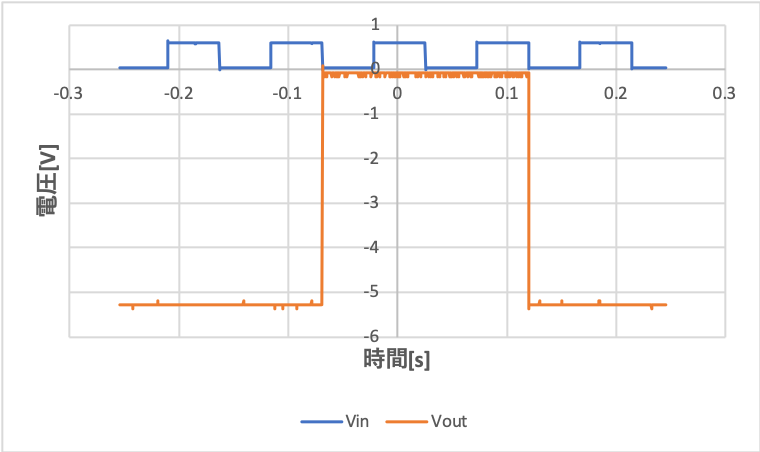
\includegraphics[width=0.8\linewidth]{fig23.png}
 \end{center}
 \caption{Q1}
 \label{fig:23}
\end{figure}

\begin{figure}[htbp]
 \begin{center}
  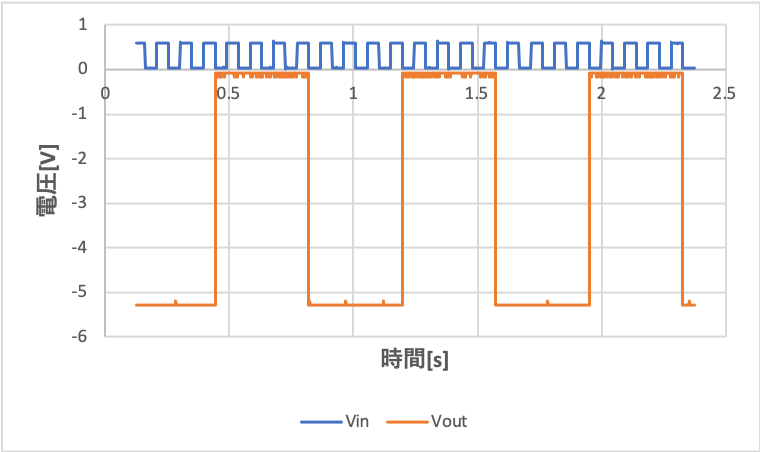
\includegraphics[width=0.8\linewidth]{fig24.png}
 \end{center}
 \caption{Q2}
 \label{fig:24}
\end{figure}

\begin{figure}[htbp]
 \begin{center}
  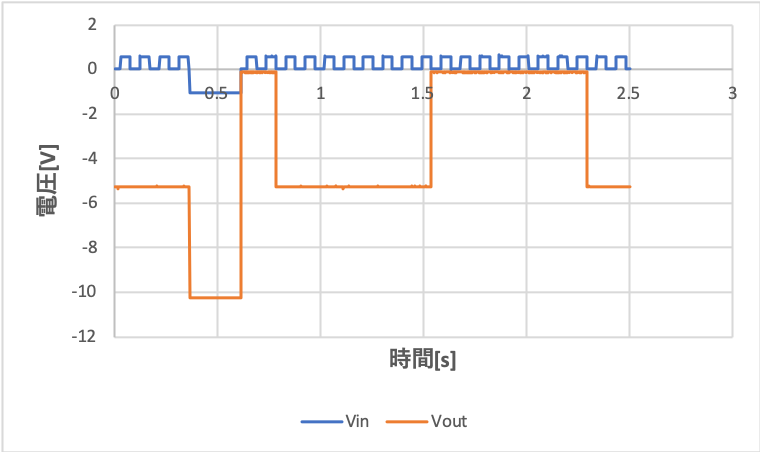
\includegraphics[width=0.8\linewidth]{fig25.png}
 \end{center}
 \caption{Q3}
 \label{fig:25}
\end{figure}

\begin{figure}[htbp]
 \begin{center}
  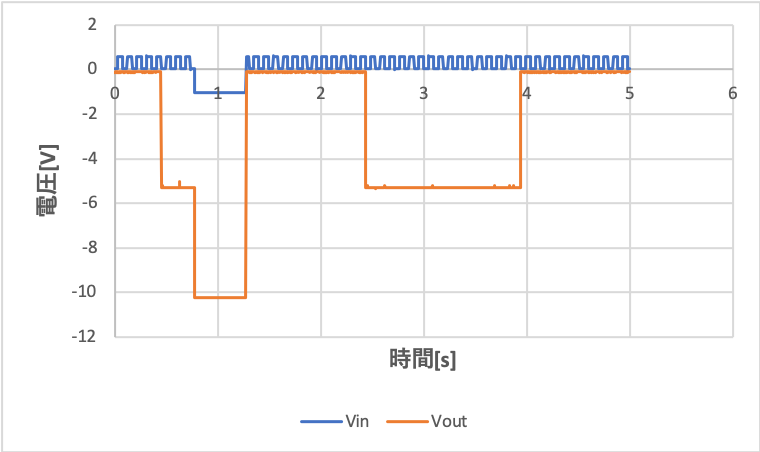
\includegraphics[width=0.8\linewidth]{fig26.png}
 \end{center}
 \caption{Q4}
 \label{fig:26}
\end{figure}

\begin{figure}[htbp]
 \begin{center}
  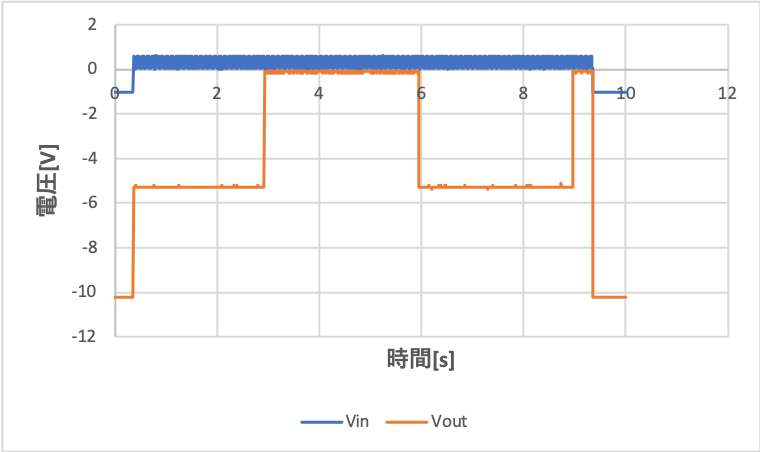
\includegraphics[width=0.8\linewidth]{fig27.png}
 \end{center}
 \caption{Q5}
 \label{fig:27}
\end{figure}


\subsubsection{Discussion}
表\ref{tab:2}からリセットセットFF回路は入力がなければ前の状態を保持し,(1,0)もしくは(0,1)の入力を受け取ると入力の状態へと遷移するシーソーのような特性を持つことが確かめられた.
また(1,1)の入力を渡すと入力後に(1,0),(0,1)のどちらかにランダムに遷移し,状態は不定となるのでフリップフロップ回路においては(1,1)入力は使うべきでないと考えられる.

また図\ref{fig:23},図\ref{fig:24},図\ref{fig:25},図\ref{fig:26},図\ref{fig:27}においてデジタルカウンター回路の出力電圧は0Vと-5Vの状態を繰り返すような動作を繰り返しており,この回数を"Count"とすると,出力電圧はファンクションジェネレーターの矩形波をCount回数えるごとに状態を遷移すると考えられる.
またCountと入力端子Qの間には以下の関係が成り立つと予想できる.
\begin{equation}
    Count = 2^{Qm} (m=1,2,...)
\end{equation}

また,図\ref{fig:25},図\ref{fig:26},図\ref{fig:27}において出力電圧に乱れがあり-10Vの出力が発生したのは出力結果をUSBで保存する際にオシロスコープのプローブの接触が悪くなり出力が乱れたことなどが考えられる.

次にカウンター回路がなぜ動作するのかについて参考文献を参照しながら考えてみる.
まず,Dフリップフロップ回路の考え方を導入して考察してみる.
そして,ファンクションジェネレーターからの矩形波入力をクロック入力と呼ぶことにする.
図\ref{fig:28}のような基本的なDF/F回路について考える.

\newpage

\begin{figure}[htbp]
 \begin{center}
  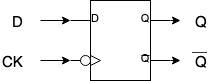
\includegraphics[width=0.8\linewidth]{fig28.png}
 \end{center}
 \caption{DF/F回路}
 \label{fig:28}
\end{figure}

この回路において真理表は以下のようになる.

\begin{table}[htb]
  \begin{center}
    \caption{DF/F回路の真理表}
    \begin{tabular}{c c c c} \hline
         $D$ & $CK$ & $Q$ & $\overline{Q}$ \\ \hline \hline
         0 & ↓ & 0 & 1 \\ \hline
         1 & ↓ & 1 & 0 \\ \hline
    \end{tabular}
    \label{tab:3}
  \end{center}
\end{table}

つまりこの回路はQを出力とすれば,クロック入力の立ち下がりにおいて入力Dの状態が出力されるという動作をする.
ここで図\ref{fig:29}のような回路について考える.

\begin{figure}[htbp]
 \begin{center}
  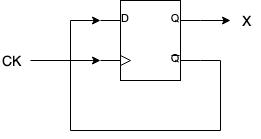
\includegraphics[width=0.8\linewidth]{fig29.png}
 \end{center}
 \caption{DF/F回路 (D=$\overline{Q}$)}
 \label{fig:29}
\end{figure}

\newpage

この回路のクロック入力に対する出力波は以下のようになる.

\begin{figure}[htbp]
 \begin{center}
  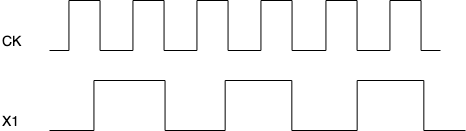
\includegraphics[width=0.8\linewidth]{fig30.png}
 \end{center}
 \caption{DF/F回路の入出力波形}
 \label{fig:30}
\end{figure}

さらに図\ref{fig:29}の回路を2個直列につなげた場合図\ref{fig:30}のXの波の立ち下がりを数えるので結果的に出力される波形はクロック入力2個分を数えて切り替わる出力となる.
またこれは実験におけるQ1の波形に他ならない.

同様に図\ref{fig:29}の回路を3個直列につなげた場合は2個直列に繋げた場合の2倍分の入力を数えて出力波を出すので結果としてはクロック入力4個分を数えて切り替わる.
以下同様にこの回路を繋げていくと2の乗数分クロック入力を数えて出力が切り替わるカウンター回路を作ることができると予想される.

ここでフリップフロップ回路の応用例について考えてみる.
フリップフロップは前の状態を保存しておくことができるのでコンピュータのメモリなどに使うことができると予想できる.

また,このカウンター回路の応用例としては周期ごとにカウントをしていくので交流電源を矩形波に変換して使えばタイマーのような時間を図ることのできる素子を形成できることが予想される.


\begin{thebibliography}{99}
\bibitem{urashimada} 松原洋平 『電気回路の基本66』 (2011)
\bibitem{oubutu} 『応用物理学実験』
\end{thebibliography}
%=============================================================
\end{document}
